% !TEX root = applied-math.tex


\chapter{Eigenvalues and Eigenvectors}

There is another very important aspect to linear algebra that will play a very important role in applied mathematics.  This is the notion of an eigenvector and eigenvalue. Briefly, these are a vector and scalar in an equation, however, first, there is a strong geometric role behind them and secondly, eigenvectors and eigenvalues play an important role in many parts of linear algebra.  Lastly, we will see an extension of them for functions later in the text.  

\section{Eigenvalues and Eigenvectors} \label{sect:eigenvalues}

\begin{definition}
 For a square matrix $A$, an \textbf{eigenvalue}\index{eigenvalue} $\lambda$ with related \textbf{eigenvector}\index{eigenvector} $\vec{v}$ satisfy
 % 
\begin{align*}
 A \vec{v} = \lambda \vec{v} 
\end{align*}
as long as $\vec{v}$ is not the zero vector.  
\end{definition}

Recall that the matrix operation $A \vec{v}$ is a linear transformation on $\vec{v}$, that is, it take a vector $\vec{v}$ to another vector.   Thus the eigenvector of a matrix is a vector such that $A\vec{v}$ results in a vector in the same direction as $\vec{v}$.  The eigenvalue is the scalar transformation associated with this. 

\begin{example}
 Show that $\vec{v}=[1\;\;1]^T$ is a eigenvector of 
 % 
\begin{align*}
 A & = 
\begin{bmatrix}
 3 & 4 \\
 2 & 5 
\end{bmatrix}
\end{align*}

\solution

We need to show that this satisfies $A \vec{v} = \lambda \vec{v}$ for some scalar $\lambda$.  Since
% 
\begin{align*}
 A \vec{v} & = 
\begin{bmatrix}
 3 & 4 \\
 2 & 5 
\end{bmatrix}
\begin{bmatrix}
 1 \\ 1 
\end{bmatrix} = 
\begin{bmatrix}
 7 \\ 7
\end{bmatrix}
\end{align*}
and since this matrix is 7 times the vector $\vec{v}$, this proves that $\vec{v}$ is an eigenvector.  The scale number 7 is the eigenvalue.  
\end{example}



\subsection{Finding Eigenvalues and Eigenvectors}

We will first find the eigenvalues of a given matrix.  
Start with the eigenvector equation:
\begin{align}
 A \vec{v} & = \lambda \vec{v}  \notag
 \intertext{subtract $\lambda \vec{v}$} 
 A \vec{v} - \lambda \vec{v} & = \vec{0},  \notag
  \intertext{introduce an identity matrix} 
 A \vec{v} - \lambda I \vec{v} & = \vec{0},  \notag
  \intertext{factor out the $\vec{v}$} 
 (A - \lambda I) \vec{v} & = \vec{0}   \label{eq:eigenvector:homo}
\end{align}
and we have transformed this into a homogeneous matrix equation.  As stated in the definition of the eigenvector, it cannot be the zero vector, and by Theorem \ref{thm:sing:matrices}, the only solution where $\vec{v}$ is nonzero is when 
% 
\begin{align}
 \det(A-\lambda I) & = 0 \label{eq:char:equation} 
\end{align}

This equation is called the characteristic equation.  

To find an eigenvector associated with the eigenvalue, solve 
% 
\begin{align*}
 (A - \lambda I) \vec{v} = \vec{0} 
\end{align*}
for $\vec{v}$, that is find the basis of the null space of the matrix $A - \lambda I$. 

Note: as we will see in all of the examples in this section that the null space of $A-\lambda I$ has at least dimension 1 and that the reduced echelon form of $A-\lambda I$ has at least one row of zeros, indicating that the rank of $A-\lambda I$ is less than $n$.   The reason for this is because of Theorem \ref{thm:sing:matrices}.  This is helpful for detecting errors in finding eigenvalues/eigenvectors.  

\begin{example} \label{ex:eigs:real1}
Find all eigenvalues\index{eigenvalue} and eigenvectors\index{eigenvector} of 
% 
\begin{align*}
\begin{bmatrix}
 3 & 4 \\
 2 & 5 
\end{bmatrix}
\end{align*}

\solution

First, solve $|A-\lambda I| = 0$, 
% 
\begin{align*}
 |A - \lambda I| & = 
\begin{vmatrix}
 3-\lambda & 4 \\
 2 & 5 - \lambda 
\end{vmatrix} = 
(3-\lambda)(5-\lambda) - 8 \\
& = \lambda^2 -8\lambda +7 = (\lambda-1)(\lambda-7) =0
\end{align*}
so $\lambda = 1,7$.  

Next, we need to find an eigenvector for each eigenvalue.  When $\lambda=1$, 
% 
\begin{align*}
 (A-1 I)\vec{v} & = 
\begin{bmatrix}
 2 & 4 \\
 2 & 4 
\end{bmatrix} \vec{v}  = 0 
\end{align*}
To solve this matrix equaiton, we'll use gaussian elimination on the augmented matrix:
% 
\begin{align*}
& \qquad \begin{bmatrix}[rr|r]
2 &4  & 0 \\
2 & 4 & 0  
\end{bmatrix} \\
-R_1 + R_2 \rightarrow R_2 & \qquad
\begin{bmatrix}[rr|r]
2 &4  & 0 \\
0 & 0 & 0  
\end{bmatrix} \\
\frac{1}{2} R_1 \rightarrow R_1 & \qquad 
\begin{bmatrix}[rr|r]
1 & 2  & 0 \\
0 & 0 & 0  
\end{bmatrix} \\
\end{align*}
The first row of the matrix corresponds to $x_1+2x_2=0$ so the null space of $A-\lambda I$ is 
% 
\begin{align*}
\{
\begin{bmatrix}
 -2 \\ 1 
\end{bmatrix} s  \; | \; s \in \mathbb{R} \}
\end{align*}
The eigenvector(s) associated with $\lambda=1$ is the basis of this space or 
% 
\begin{align*}
 \vec{v} & = 
\begin{bmatrix}
 -2 \\ 1 
\end{bmatrix}
\end{align*}


And to find the eigenvector associated with $\lambda = 7$, solve
% 
\begin{align*}
 (A - 7 I) \vec{v} & = 
\begin{bmatrix}
 -4 & 4 \\
 2 & -2 
\end{bmatrix} \vec{v} = \vec{0} 
\end{align*}
and use Gaussian Elimination to reduce
% 
\begin{align*}
 & \qquad \begin{bmatrix}[rr|r]
 -4 & 4 & 0 \\
 2 & -2 & 0 
\end{bmatrix} \\
\begin{array}{r}
-\frac{1}{4} R_1 \rightarrow R_1  \\
-2 R_1 + R_2 \rightarrow R_2  
\end{array} & \qquad
\begin{bmatrix}[rr|r]
1 & -1 & 0 \\
0 & 0 & 0  
\end{bmatrix}
\end{align*}
The null space of $A-7I$ is 
% 
\begin{align*}
\{
\begin{bmatrix}
 1 \\ 1 
\end{bmatrix} s \; | \; s \in \mathbb{R} \}
\end{align*}
so the eigenvector associated with $\lambda=7$ is the basis of this space or 
% 
\begin{align*}
 \vec{v} & = 
\begin{bmatrix}
 1 \\ 1 
\end{bmatrix}
\end{align*}

Overall, there are two eigenvalues and two related eigenvectors they are 
%
\begin{align*}
\lambda_1 & = 1, \quad \vec{v}_1 = \begin{bmatrix}
-2 \\1 
\end{bmatrix} & 
\lambda_2 & = 7, \quad \vec{v}_2 = \begin{bmatrix}
1 \\1 
\end{bmatrix} 
\end{align*}

\end{example}

This example showed that this $2 \times 2$ matrix has two real eigenvalues and two corresponding eigenvectors.  Also, although it seemed that these eigenvectors may be unique, we'll show that $[-3\;\;-3]^{\intercal}$ is also a eigenvector of the matrix in Example \ref{ex:eigs:real1}.  
%
\begin{align*}
\begin{bmatrix}
3 & 4 \\ 2 & 5 
\end{bmatrix}\begin{bmatrix}
-3 \\ -3 
\end{bmatrix} & = \begin{bmatrix}
-21 \\ -21 
\end{bmatrix} = 7 \begin{bmatrix}
-3 \\ -3
\end{bmatrix}
\end{align*}
which shows directly that $[-3\;\;-3]^{\intercal}$ is an eigenvector with corresponding eigenvalue 7.  Does this mean that there are other eigenvectors?  Yes.  The following lemma shows this. 

\begin{lemma} \label{lem:eigenvector:scale}
If $\vec{v}$ is an eigenvector of $A$ with corresponding eigenvalue $\lambda$, then $k\vec{v}$ is also an eigenvector of $A$ with corresponding eigenvalue $\lambda$ if $k \neq 0$. 
\end{lemma}

\begin{proof}
Since $\vec{v}$ is an eigenvector of $A$ with corresponding eigenvalue $\lambda$, then $A \vec{v} = \lambda \vec{v}$.  Multiplying this by $k$ results in
%
\begin{align*}
k(A \vec{v}) & = k (\lambda \vec{v}) \\
A (k \vec{v}) & = \lambda (k \vec{v})
\end{align*}
which shows the result.  Also note, that $k$ cannot be zero, because $0\vec{v}$ is the zero vector, which is not an eigenvector.  
\end{proof}




There are other possibilities of eigenvalues and eigenvectors of $2 \times 2$ matrices.    The following has complex eigenvalues.  



\begin{example} \label{ex:eigs:complex} 
Find the eigenvalues\index{eigenvalue} and eigenvectors\index{eigenvector} of 
%
\begin{align*}
\begin{bmatrix}
0 & 2 \\ -2 & 0
\end{bmatrix}
\end{align*}

To find the eigenvalues, we find
%
\begin{align*}
\begin{vmatrix}
-\lambda & 2 \\ -2 & -\lambda 
\end{vmatrix} = 0
\end{align*}
%
or $\lambda^2 + 4 =0$, which has the solutions $\lambda = \pm 2i$.  

To find the eigenvectors, we find the null space associated with each of the two eigenvalues.  

\textbf{Eigenvector for $\lambda = 2i$}

Find the null space of $A-2iI$: 
%
\begin{align*}
& \qquad \begin{bmatrix}
-2i & 2 \\ -2 & -2i
\end{bmatrix} \\
\frac{1}{-2i} R_1 \rightarrow R_1 
& \qquad \begin{bmatrix}
1 & i \\ -2 & -2i
\end{bmatrix} \intertext{where $\frac{-2}{2i}=\frac{-1}{i} =\frac{-i}{i^2}=\frac{-i}{-1}=i$ is used} 
2R_1 + R_2 \rightarrow R_2, & \qquad
\begin{bmatrix}
1 & i \\ 0 & 0
\end{bmatrix}
\end{align*}
and the top equation says $x_1 = - ix_2$, so the null space is
%
\begin{align*}
\{ \begin{bmatrix}
-i \\ 1 
\end{bmatrix}x_2 \; | \; x_2 \in \mathbb{R} \}
\end{align*}
so the eigenvector is $[-i \; \; 1]^{\intercal}$. 

\textbf{Eigenvector for $\lambda = -2i$}

Find the null space of $A-2iI$: 
%
\begin{align*}
& \qquad \begin{bmatrix}
2i & 2 \\ -2 & 2i
\end{bmatrix} \\
\frac{1}{2i} R_1 \rightarrow R_1 
& \qquad \begin{bmatrix}
1 & -i \\ -2 & -2i
\end{bmatrix} \\
2R_1 + R_2 \rightarrow R_2, & \qquad
\begin{bmatrix}
1 & -i \\ 0 & 0
\end{bmatrix}
\end{align*}
and the top equation says $x_1 = ix_2$, so the null space is
%
\begin{align*}
\{ \begin{bmatrix}
i \\ 1 
\end{bmatrix}x_2 \; | \; x_2 \in \mathbb{R} \}
\end{align*}
so the eigenvector is $[i \; \; 1]^{\intercal}$. 
\end{example}

Notice in the last example that there where complex conjugate pairs of eigenvalues and associated eigenvectors.  This always occurs with a real matrix $A$.  The following theorem summarizes this. 

\begin{theorem}
Let $A$ be a real matrix.  If $\lambda$ is an complex eigenvalue\index{eigenvalue} with corresponding eigenvector\index{eigenvector}, $\vec{v}$, then the complex conjugate of $\lambda,$ denoted $\overline{\lambda}$ is also an eigenvalue with corresponding complex conjuate eigenvector $\overline{\vec{v}}$.
\end{theorem}

\begin{proof}
If $\lambda$, $\vec{v}$ is an eigenvalue-eigenvector pair of $A$, then 
%
\begin{align*}
A\vec{v} = \lambda \vec{v}
\end{align*}
And taking the complex conjugate of this equation.  
\begin{align*}
\overline{A\vec{v}} & = \overline{\lambda \vec{v}} \\
A \overline{\vec{v}} & = \overline{\lambda} \, \overline{\vec{v}}
\end{align*}
where $\overline{A}=A$ because $A$ is real.  This shows that $\overline{\lambda}$, $\overline{\vec{v}}$ is a eigenvalue-eigenvector pair of $A$.  

\end{proof}

The result of this theorem will save work if you have a real matrix and find a complex eigenvalue.  For example in Example \ref{ex:eigs:complex}, the first eigenvalue-eigenvector pairs was $\lambda_1=2i$ and $\vec{v}_1=[-i \; \; 1]^{\intercal}$.  The above theorem shows that $\lambda_2=\overline{\lambda_1} = -2i$ and $\vec{v}_2=\overline{\vec{v}_1} = [i \; \; 1]^{\intercal}$ is another eigenvalue-eigenvector pair.  

The next example has real eigenvalue and eigenvector, but has a different feature than Example \ref{ex:eigs:real1}.  

\begin{example}
Find the eigenvalues\index{eigenvalue} and eigenvectors\index{eigenvector} of 
%
\begin{align*}
\begin{bmatrix}
2 & -1 \\ 1 & 4
\end{bmatrix}
\end{align*}

\solution

The eigenvalues are found by solving the characteristic equation 
%
\begin{align*}
|A-\lambda I| & = \begin{vmatrix}
2-\lambda & -1 \\ 1 & 4-\lambda
\end{vmatrix} = (2-\lambda)(4-\lambda)+1 \\
& = \lambda^2-6\lambda + 9 
\end{align*}
And solving $|A-\lambda I|=0$ has the single root $\lambda = 3$.  To find the associated eigenvector, we solve for the null space of $A-3I$ 

\begin{align*}
A-3I = & \begin{bmatrix}
-1 & -1 \\
1 & 1 
\end{bmatrix} \\
R_1 + R_2 \rightarrow R_2 \qquad & \begin{bmatrix}
-1 & -1 \\
0 & 0 
\end{bmatrix}
\end{align*}
which has the only equation $-x_1 = x_2$ or $x_1 =-x_2$ which shows that the null space is
%
\begin{align*}
\{ \begin{bmatrix}
-1 \\ 1 
\end{bmatrix} x_2 \; | \; x_2 \in \mathbb{R} \}
\end{align*}
and the eigenvector is $\vec{v} = [-1\;\; 1]^{\intercal}$.   
\end{example}

And this next example has only one eigenvalue however has two linearly independent eigenvectors.  

\begin{example} \label{ex:eigs:scale2}
Find the eigenvalues\index{eigenvalue} and eigenvectors\index{eigenvector} of 
%
\begin{align*}
\begin{bmatrix}
2 & 0 \\ 0 & 2
\end{bmatrix}
\end{align*}

This has the characteristic equation $(\lambda-2)^2 = 0$ or the single root $\lambda = 2$.  

To find the eigenvectors we find the null space of $A-2I$ or 
%
\begin{align*}
\begin{bmatrix}
0 & 0 \\ 0 & 0 
\end{bmatrix} 
\end{align*}
%
and any vector in $\mathbb{R}^2$ is in the null space.  We can write down the space using the standard basis vectors 
%
\begin{align*}
\{ \begin{bmatrix}
1 \\ 0 
\end{bmatrix} x_1 + \begin{bmatrix}
0 \\ 1
\end{bmatrix} x_2 \;|\; x_1, x_2 \in \mathbb{R} \}
\end{align*}
so $\vec{v}_1 = [1\;\;0]^{\intercal}$ and $\vec{v}_2=[0\; \;1]^{\intercal}$ are both eigenvectors associated with $\lambda=2$.  
\end{example}

\subsection*{Possible Eigenvalue/Eigenvector combinations of a $2\times 2$ matrix}

In the previous examples, we have seen the following:
%
\begin{itemize}
\item 2 real eigenvalues, 2 linearly independent eigenvectors 
\item 2 complex eigenvalues (complex conjugates) and 2 linearly indepedent eigenvectors (complex conjugates).  
\item 1 real eigenvalue, 2 linearly independent eigenvectors
\item 1 real eigenvalue, 1 eigenvector.
\end{itemize}

In fact, these are the possibilities for any 2 by 2 real matrix.   We now examine two examples of the eigenvalues/eigenvectors of 3 by 3 matrices.  


\begin{example} \label{ex:eigs:3by3}
Find the eigenvalues and eigenvectors of the 3 by 3 matrix
%
\begin{align*}
\begin{bmatrix}
1 & 0 & 0 \\
3 & -2 & 6 \\
2 & 1 & 3
\end{bmatrix}
\end{align*}

\solution

To find the eigenvalues, we solve the characteristic equation $|A-\lambda I|=0$ or expanding across the first row to find the determinant and we solve
%
\begin{align*}
|A-\lambda I| &= \begin{vmatrix}
1-\lambda & 0 & 0 \\
3 & -2-\lambda & 6 \\
2 & 1 & 3-\lambda
\end{vmatrix} = (1-\lambda) \begin{vmatrix}
-2 - \lambda & 6 \\ 1 & 3-\lambda 
\end{vmatrix} \\
&=(1-\lambda)( (-2-\lambda)(3-\lambda) -6) =0
\end{align*} 
which has roots $\lambda=1,4,-3$.

To find the corresponding eigenvectors, we solve for the null space of $A-\lambda I$ for each $\lambda$
\begin{description}
\item[$\lambda=1$] 

\begin{align*}
A-I = & \begin{bmatrix}
0 & 0 & 0 \\
3 & -3 & 6 \\
2 & 1 & 2
\end{bmatrix} \\
\begin{array}{r}
R_2 \leftrightarrow R_1\\
R_3 \leftrightarrow R_2 
\end{array}
 \qquad & 
\begin{bmatrix}
3 & -3 & 6 \\
2 & 1 & 2\\
0 & 0 & 0 \\
\end{bmatrix} \\
\frac{1}{3} R_1 \rightarrow R_1 \qquad & 
\begin{bmatrix}
1 & -1 & 2 \\
2 & 1 & 2\\
0 & 0 & 0 \\
\end{bmatrix} \\
-2 R_1 + R_2 \rightarrow R_2 \qquad & 
\begin{bmatrix}
1 & -1 & 2 \\
0 & 3 & -2\\
0 & 0 & 0 \\
\end{bmatrix}\\
R_2 + 3R_1 \rightarrow R_1 \qquad & 
\begin{bmatrix}
3 & 0 & 4 \\
0 & 3 & -2\\
0 & 0 & 0 \\
\end{bmatrix}
\end{align*}
and other that a factor of 3, this is in reduced row echelon form.  The top two equations are
%
\begin{align*}
x_1 & = -\frac{4}{3} x_3 \\
x_2 & = \frac{2}{3} x_3
\end{align*}
and the null space is
%
\begin{align*}
\begin{bmatrix}
-4/3 \\ 2/3 \\ 1
\end{bmatrix} x_3 \; | \; x_3
\end{align*}
And we could take $[-4/3\;\;2/3\;\; 1]^{\intercal}$ as an eigenvector, however, from Lemma \ref{lem:eigenvector:scale}, a scalar multiple of an eigenvector is also an eigenvector, so multiplying by 3 results in $\vec{v}_1=[-4\;\;2\;\;3]^{\intercal}$.

\item[$\lambda=4$]

\begin{align*}
A-4I = & \begin{bmatrix}
3 & 0 & 0 \\
3 & -6 & 6 \\
2 & 1 & -1
\end{bmatrix} \\
\frac{1}{3} R_1 \rightarrow R_1 \qquad &
\begin{bmatrix}
1 & 0 & 0 \\
3 & -6 & 6 \\
2 & 1 & -1
\end{bmatrix} \\
\begin{array}{r}
-3R_1 + R_2 \rightarrow R_2 \\
-2R_1 + R_3 \rightarrow R_3 
\end{array} \qquad & 
\begin{bmatrix}
1 & 0 & 0 \\
0 & -6 & 6 \\
0 & 1 & -1 
\end{bmatrix} \\
-\frac{1}{6} R_2 \rightarrow R_2 \qquad & 
\begin{bmatrix}
1 & 0 & 0 \\
0 & 1 & -1 \\
0 & 1 & -1 
\end{bmatrix} \\
-R_2 + R_3 \rightarrow R_3 \qquad &
\begin{bmatrix}
1 & 0 & 0 \\
0 & 1 & -1 \\
0 & 0 & 0 
\end{bmatrix} \\
\end{align*}
%
and the top two equations are $x_1=0$ and $x_2=x_3$ so the null space can be written
%
\begin{align*}
\{ \begin{bmatrix}
0 \\ 1 \\ 1
\end{bmatrix} x_3 \; |\; x_3 \in \mathbb{R} \}
\end{align*}
so the eigenvectors is $[0\;\;1\;\;1]^{\intercal}$.  

\item[$\lambda=-3$]

\begin{align*}
A+3I = &\begin{bmatrix}
4 & 0 & 0 \\
3 & 1 & 6 \\
2 & 1 & 6
\end{bmatrix}\\
\frac{1}{4} R_1 \rightarrow R_1 \qquad & 
\begin{bmatrix}
1 & 0 & 0 \\
3 & 1 & 6 \\
2 & 1 & 6
\end{bmatrix}\\
\begin{array}{r}
-3R_1 + R_2 \rightarrow R_2 \\
-2R_1 + R_3 \rightarrow R_3 
\end{array} \qquad &
\begin{bmatrix}
1 & 0 & 0 \\
0 & 1 & 6 \\
0 & 1 & 6
\end{bmatrix}\\
-R_2 + R_3 \rightarrow R_3 \qquad & 
\begin{bmatrix}
1 & 0 & 0 \\
0 & 1 & 6 \\
0 & 0 & 0 
\end{bmatrix}
\end{align*}
%
and the top two equations are $x_1=0$, $x_2=-6x_3$ so the null space is
%
\begin{align*}
\{ \begin{bmatrix}
0 \\ -6 \\ 1
\end{bmatrix} x_3 \; | \; x_3 \in \mathbb{R} \}
\end{align*}
Therefore the eigenvector is  $\vec{v}_3=[0\;\;-6\;\;1]^{\intercal}$.  

\end{description}

\end{example}

\begin{example}
Find the eigenvalues and eigenvectors of 
%
\begin{align*}
A & = \begin{bmatrix}
1 & 0 & 2 \\
2 & 0 & 4 \\
-1 & 0 & -2 
\end{bmatrix}
\end{align*}

\solution

First, we solve for the eigenvectors by solving $|A-\lambda I|=0$, 
%
\begin{align*}
|A-\lambda I| & = \begin{vmatrix}
1-\lambda & 0 & 2 \\
2 & -\lambda & 4 \\
-1 & 0 & -2- \lambda 
\end{vmatrix} \\
& = -\lambda \begin{vmatrix}
1-\lambda & 2 \\
-1 & -2-\lambda 
\end{vmatrix} = -\lambda \bigl( (1-\lambda)(-2-\lambda)+2 \bigr) \\
& = -\lambda (\lambda^2 - \lambda -2 + 2)  = -\lambda^3 - \lambda^2 
\end{align*}
and this is 0, when $\lambda=0$ and $\lambda = -1$.  

Next, find the eigenvectors. The eigenvectors with $\lambda=0$ are found by finding the null space of $A-0I$:
%
\begin{align*}
& \qquad \begin{bmatrix}
1 & 0 & 2 \\
2 & 0 & 4 \\
-1 & 0 & -2
\end{bmatrix} \\
\begin{array}{r}
-2R_1 + R_2 \rightarrow R_2 \\
R_1+R_3 \rightarrow R_3 
\end{array}
& \qquad 
\begin{bmatrix}
1 &0 & 2 \\
0 & 0 & 0 \\
0 & 0 & 0 
\end{bmatrix}
\end{align*}
and since the only equation is $x_1 +2x_3=0$, both $x_2$ and $x_3$ are free variables and the solution space (therefore the null space) can be written:
%
\begin{align*}
\{ \begin{bmatrix}
0 \\ 1 \\ 0
\end{bmatrix} x_2 + \begin{bmatrix}
-2 \\ 0 \\ 1
\end{bmatrix} x_3 \; | \; x_2, x_3 \in \mathbb{R} \} 
\end{align*}
This shows that the vectors 
%
\begin{align*}
\vec{v}_1 & = \begin{bmatrix}
0 \\ 1\\ 0
\end{bmatrix}&  \vec{v}_2 & = \begin{bmatrix}
-2 \\ 0 \\ 1
\end{bmatrix} 
\end{align*}
are both eigenvectors associated with $\lambda=0$.  The eigenvectors associated with $\lambda = -1$ is found by seeking the null space of $A-I$:
%
\begin{align*}
& \qquad \begin{bmatrix}
2 & 0 & 2 \\
2 & 1 & 4 \\
-1 & 0 & -1 
\end{bmatrix} \\
\frac{1}{2}R_1 \rightarrow R_1 & \qquad
\begin{bmatrix}
1 & 0 & 1 \\
2 & 1 & 4 \\
-1 & 0 & -1 
\end{bmatrix} \\
\begin{array}{r}
-2R_1 + R_2 \rightarrow R_2, \\
R_1 + R_3 \rightarrow R_3,
\end{array}
& \qquad \begin{bmatrix}
1 & 0 & 1 \\
0 & 1 & 2 \\
0 & 0 & 0 
\end{bmatrix}
\end{align*}
These equations are 
%
\begin{align*}
x_1 & = -x_3 \\
x_2 & = -2x_3 
\end{align*}
so the solution set (and the null space) is
%
\begin{align*}
\{ \begin{bmatrix}
-1 \\ -2 \\ 1
\end{bmatrix} x_3 \; \ \; x_3 \in \mathbb{R} \} 
\end{align*}
so the eigenvector associated with $\lambda_3 =-1$ is
%
\begin{align*}
\begin{bmatrix}
-1 \\ -2 \\ 1
\end{bmatrix}
\end{align*}
\end{example}


\section{Eigenvalues and  Linear Maps}

Recall that in section \ref{sect:eigenvalues} that the eigenvalues and eigenvectors of a square matrix was found. We will examine how we can find eigenvalues and eigenvectors of a linear map.  The definition of these are extensions of what we saw for matrices.

\begin{definition}
Let $T:V \rightarrow V$ be a linear map and $V$ be a finite dimensional vector space.  The nonzero vector $\vec{x}$ is an \textbf{eigenvector} with associated \textbf{eigenvalue} if
%
\begin{align*}
T(\vec{x}) = \lambda \vec{x}
\end{align*}
\end{definition}

There are a few ways to find $\vec{x}$ and $\lambda$.  In this section, we'll only see some examples that are relatively simple to see as well as finding the matrix representation of the map.  In addition, this section only shows examples from finite dimensional vector spaces, however, in general, there is no restriction.  

For the remainder of this chapter we will see examples of eigenvalues and eigenvectors of linear maps, including rotations, scales and derivative maps.  We first see an example of scaling a vector in $\mathbb{R}^2$.  

\begin{example}

Find the eigenvalues and eigenvectors of the scale map $S$ from Example \ref{ex:scale:map}.  

\solution

Recall that the scale map $S: \mathbb{R}^2 \rightarrow \mathbb{R}^2$ is given by 
%
\begin{align*}
S(\vec{x}) = k \vec{x}
\end{align*}

To find the eigenvalues and eigenvectors of $S$, we seek an $\vec{x}$ and a $\lambda$ such that 
%
\begin{align*}
S(\vec{x})=\lambda \vec{x}
\end{align*}
but since $S(\vec{x})=k \vec{x}$, then $\lambda =k$ and any $\vec{x}$ is an eigenvector.  

Alternatively, we can write down the matrix $A_S$ associated with the map.  This was done in Example \ref{ex:scale:map:matrix:rep} and is
%
\begin{align*}
A_S & = \begin{bmatrix}
k & 0 \\ 0 & k 
\end{bmatrix}
\end{align*}
The eigenvalues and eigenvectors of this was found in Example \ref{ex:eigs:scale2} for a particular $k$, but generalizing that, one can see that $\lambda=k$ will be the only eigenvector of $A_S$ with eigenvectors $[1\;\;0]^{\intercal}$ and $[0\;\;1]^{\intercal}$.  

In this case, since there are two eigenvectors associated with $\lambda=k$, any linear combination of the two eigenvectors is also an eigenvector, and since $[1\;\;0]^{\intercal}$ and $[0\;\;1]^{\intercal}$ span $\mathbb{R}^2$, any vector in $\mathbb{R}^2$ is an eigenvector.  
\end{example}

The next example shows the eigenvalues of the linear map associated with a derivative.  

\begin{example}
The set 
%
\begin{align*}
V & = \{ ae^{x} + b e^{-x} \; | \; a,b \in \mathbb{R} \}
\end{align*}
is a subspace of all functions on $\mathbb{R}$.  A basis for this subspace is $(e^x,e^{-x})$.  In addition, the differential operation $D:V \rightarrow V$ is a linear transformation.   What are the eigenvalues and eigenvectors of $D$?  

\solution

There are two ways of looking at this.  Since $e^{x} \mapsto e^x$, this means that $e^x$ is an eigenvector with corresponding eigenvalue 1.  Similarly, since $e^{-x} \mapsto -e^{-x}$, this also means that $e^{-x}$ is an eigenvector with eigenvalue $-1$.  

Alternatively, this can be done by first finding the matrix representation of the differential operator or
%
\begin{align*}
A_D & = \begin{bmatrix}
1 & 0 \\
0 & -1 
\end{bmatrix}
\end{align*}
Recall that in the case of diagonal matrices, the eigenvalues are on the diagonal or $\lambda_1=1$ and $\lambda_2=-1$.  One can also find that the corresponding eigenvectors are 
%
\begin{align*}
\vec{v}_1 & = \begin{bmatrix}
1 \\ 0 
\end{bmatrix} & \vec{v}_2 & = \begin{bmatrix}
0 \\ 1 
\end{bmatrix}
\end{align*}
These two vectors can be translated back to the functional forms $e^{x}$ and $e^{-x}
$, the same as we found above.  These two functions which are in $V$ are functions that stay the same in the subspace $V$ up to a scalar constant.  


\end{example}

\vspace{2in}

\begin{example}
Consider the differential map $D: \mathcal{P}_3 \rightarrow \mathcal{P}_3$ which maps cubic polynomials to other cubic polynomials. 

\begin{align*}
A & = \begin{bmatrix}
0 & 1 & 0 & 0 \\
0 & 0 & 2 & 0 \\
0 & 0 & 0 & 3 \\
0 & 0 & 0 & 0 
\end{bmatrix}
\end{align*}

Find the eigenvalues of this matrix and interpret. 

\solution

First, we find the determinant of 
%
\begin{align*}
|A-\lambda I| & = \begin{vmatrix}
-\lambda & 1 & 0 & 0 \\
0 & -\lambda & 2 & 0 \\
0 & 0 & -\lambda & 3 \\
0 & 0 & 0 & -\lambda 
\end{vmatrix} = (-\lambda)^4 
\end{align*}
and setting it to zero, thus $\lambda=0$ is the only eigenvalue.  To find the eigenvectors, we find the null space of the original matrix, which after scaling the second and third row, the matrix is the reduced row echelon form:
%
\begin{align*}
 \begin{bmatrix}
0 & 1 & 0 & 0 \\
0 & 0 & 1 & 0 \\
0 & 0 & 0 & 1 \\
0 & 0 & 0 & 0 
\end{bmatrix}
\end{align*}
and the solution to the null space is
%
\begin{align*}
\{ \begin{bmatrix}
1 \\ 0 \\ 0 \\ 0
\end{bmatrix} s \; | \; s \in \mathbb{R} \} 
\end{align*}

This vector is the representation of the cubic polynomial $p(x)=c$, a constant.   Thus, the only vector that remains the same under differentiation is the constant polynomial with eigenvalue 0.  

\end{example}


For the last example in this section, consider the map that rotates a 2 by 2 matrix 90$^{\circ}$ clockwise.  That is $R: \mathcal{M}_{2 \times 2} \rightarrow \mathcal{M}_{2 \times 2}$ such that 
%
\begin{align*}
\begin{bmatrix}
a & b \\
c & d 
\end{bmatrix} \mapsto \begin{bmatrix}
c & a \\ d& b 
\end{bmatrix}
\end{align*}
One can show that if we consider the vector representation in the basis:
%
\begin{align*}
B & = \biggl( \begin{bmatrix}
1 &0 \\ 0 & 0 
\end{bmatrix}, \begin{bmatrix}
0 &1 \\ 0 & 0 
\end{bmatrix}, \begin{bmatrix}
0 &0 \\ 1 & 0 
\end{bmatrix}, \begin{bmatrix}
0 &0 \\ 0 & 1
\end{bmatrix} \biggr) 
\end{align*}
that
%
\begin{align*}
\text{Rep}_B \biggl( \begin{bmatrix}
a & b \\ c & d 
\end{bmatrix} \biggr) = \begin{bmatrix}
a \\ b \\ c \\ d
\end{bmatrix}
\end{align*}
and the map $R$ can be represented by the matrix as
%
\begin{align*}
A_R & = \begin{bmatrix}
0 & 1 & 0 & 0 \\
0 & 0 & 0 & 1 \\
1 & 0 & 0 & 0 \\
0 & 0 & 1 & 0 
\end{bmatrix}
\end{align*}

We now find the eigenvalues and eigenvectors of this.  The eigenvalue-ei\-gen\-vector pairs are
%
\begin{align*}
\lambda_1 & = 1 & \vec{v}_1 & = \begin{bmatrix}
1 \\ 1 \\ 1 \\1 
\end{bmatrix} & \lambda_2 & = -1 & \vec{v}_2 & = \begin{bmatrix}
1 \\ -1 \\ -1 \\ 1 
\end{bmatrix}, \\
\lambda_3 & = i & \vec{v}_3 & = \begin{bmatrix}
1 \\ -i \\ i \\ -1 
\end{bmatrix} & \lambda_4 & = -i &  \vec{v}_4 & = \begin{bmatrix}
1 \\ i \\ -i \\ -1 
\end{bmatrix}
\end{align*}

To translate this back to the map that rotates the matrix, we translate each of the eigenvectors to the matrix that it represents.  For example, $\vec{v}_1$ is the matrix 
%
\begin{align*}
\begin{bmatrix}
1 & 1 \\ 1 & 1
\end{bmatrix}
\end{align*}
and if that matrix is rotated, you get it back and the eigenvector is 1.  The second eigenvector can be written as the matrix 
%
\begin{align*}
\begin{bmatrix}
1 & -1 \\ -1 & 1 
\end{bmatrix}
\end{align*}
and if you rotate this matrix, you get the matrix %
\begin{align*}
\begin{bmatrix}
-1& 1 \\ 1 & -1 
\end{bmatrix}
\end{align*}
which is the above matrix multiplied by the eigenvalue $\lambda_2=-1$.  In other words:
%
\begin{align*}
R\biggl(
\begin{bmatrix}
1 & -1 \\ -1 & 1 
\end{bmatrix} \biggr) & = -
\begin{bmatrix}
1 & -1 \\ -1 & 1 
\end{bmatrix}
\end{align*}

The other two work in a similar manner, however complex numbers are needed.  

%\section[Symmetric Matrices\ldots]{Symmetric and Orthogonal Matrices and Quadratic Forms}
%
%
%\begin{definition}
%A square matrix $A$ is said to be \textbf{symmetric} if $A=A^T$.
%\end{definition}
%
%\begin{theorem}
% The eigenvalues of a symmetric matrix are real.  
%\end{theorem}
%
%\begin{proof}
%Let $\lambda$ be an eigenvalue of $A$ with corresponding eigenvector $\vec{v}$.  
%
%\begin{align*}
%A \vec{v} & = \lambda \vec{v}  \intertext{Right multiply by $\vec{v}^T$} 
%\vec{v}^T A \vec{v}  & = \lambda \vec{v}^T \vec{v} 
%\end{align*}
%
%Take the complex conjugate of the eigenvector equation above:
%% 
%\begin{align*}
%\overline{\vec{v}}^T A^T & = \overline{\lambda} \overline {\vec{v}}^T \\
%\overline{\vec{v}}^T A & = \overline{\lambda} \overline {\vec{v}}^T \intertext{left mulitply by $\vec{v}$} 
%\overline{\vec{v}}^T A \vec{v} & = \overline{\lambda} \overline{\vec{v}}^T \vec{v} \\
%\overline{\vec{v}}^T \lambda \vec{v} & = \overline{\lambda} \overline{\vec{v}}^T \vec{v} \\
%\lambda \overline{\vec{v}}^T \vec{v} & = \overline{\lambda} \overline{\vec{v}}^T \vec{v} 
%\end{align*}
%so $\lambda = \overline{\lambda}$, hence it is real.  
%\end{proof}
%
%\begin{theorem}
%The eigenvectors of a symmetric matrix are orthogonal.  
%\end{theorem}
%
%
%\begin{definition}
%A square matrix $Q=[\vec{q}_1\;\; \vec{q}_2\;\;\vec{q}_3\;\; \cdots\;\;\vec{q}_n] $ is said to be \textbf{orthogonal} if 
%%
%\begin{align*}
%\vec{q}_i^T \vec{q}_j = 0 
%\end{align*}
%for all $i \neq j$.  If in addition that $\vec{q}_i^T\vec{q}_i = 1$ for all $i$ then the matrix is also said to be \textbf{orthonormal}.  
%\end{definition}
%
%\begin{theorem}
%If $Q$ is a orthonormal matrix, then $Q^T = Q^{-1}$.  
%\end{theorem}
%
%\subsection{Orthogonal Transformations}  
%
%Let $Q$ be a linear transformation from $\mathbb{R}^n$ to $\mathbb{R}^n$.  If $Q$ is an orthonormal matrix, then the linear transformation is said to be an \textbf{orthogonal transformation}. 
%
%\begin{example}
%Show that the rotational transformation given in section 7.10 is an orthogonal transformation. 
%
%\solution
%
%Show that 
%% 
%\begin{align}
%Q & = \begin{bmatrix}
%\cos \theta & -\sin \theta \\
%\sin \theta & \cos \theta
%\end{bmatrix}
%\end{align}
%satisfies $Q^T = Q^{-1}$.  
%\end{example}
%
%\begin{definition}
%A \textbf{quadratic form} is a polynomial function in $x_1, x_2, \ldots, x_n$ such that 
%%
%\begin{align*}
%q(\vec{x})  & = a_1 x_1^2 + a_2 x_2^2 + \cdots a_n x_n^2 + b_{12} x_1 x_2 + b_{13} x_1 x_3 + \cdots
%\end{align*}
%\end{definition}
%
%Note that a quadratic form can have squared terms and products between only two variables.  
%
%
%\begin{example}
%The following are examples of quadratic forms.  
%\begin{itemize}
%\item $4x_1^2 + 7x_2^2 + 4x_1x_2$
%\item $x_1^2 + 4x_2^2 + 9 x_3^2 -2x_1x_2 + 3x_1x_3 + x_2x_3 $
%\end{itemize}
%And the following are not:
%\begin{itemize}
%\item $x_1^2 + 4x_2^2 + 9x_2+ 3$.  
%\item $x_1^2 + 4x_2^2 + 3x_3^2 + 2x_1x_2 -3x_1 x_2 x_3 $.  
%\end{itemize}
%\end{example}
%
%A quadratic form can be written as 
%% 
%\begin{align*}
%q(\vec{x}) & = \vec{x}^T A \vec{x}
%\end{align*}
%for some symmetric matrix $A$ and $\vec{x}=[x_1\;\; x_2 \;\; \cdots \;\; x_n]^T$.  
%
%\begin{example}
%Find the matrix $A$ for the quadratic forms above:
%
%\solution
%
%\begin{align*}
%A &= \begin{bmatrix}
%4 &2 \\
%2 & 7 
%\end{bmatrix} \\
%\vec{x}^T A \vec{x} & = [x_1 \;\; x_2] \begin{bmatrix}
%4 &2 \\
%2 & 7 
%\end{bmatrix} \begin{bmatrix}
%x_1 \\ x_2 
%\end{bmatrix} \\
%& = [x_1 \;\; x_2] \begin{bmatrix}
%4x_1 + 2 x_2 \\
%2 x_1 + 7 x_2 
%\end{bmatrix}\\
%& = 4x_1^2 + 2 x_1 x_2 + 2 x_1 x_2 + 7 x_2^2 
%\end{align*}
%
%And for the second quadratic form: 
%
%\begin{align*}
%A & = \begin{bmatrix}
%1 & -1 & 3/2 \\
%-1 & 4 & 1/2 \\
%3/2 & 1/2 & 9 
%\end{bmatrix}
%\end{align*}
%\end{example}
%
%\subsection{Principle Axes of Quadratic Forms}
%
%For the quadratic form:
%% 
%\begin{align*}
%q(\vec{x}) & = \vec{x}^T A \vec{x} 
%\end{align*}
%if $A = P D P^{-1}$ can be written:
%% 
%\begin{align*}
%q(\vec{x}) & = \vec{x}^T P D P^{-1} \vec{x} \intertext{and since $A$ is symmetric then the eigenvectors form an orthonormal basis so $P^{-1} = P^T$.}  
%q(\vec{x}) & = \vec{y}^T D \vec{y}
%\end{align*}
%where $\vec{y}= P^T \vec{x}$.  
%
%
%Example of ellipse/contour plot.  

\section[Applications]{Applications of Eigenvalues and Eigenvectors}

We will develop a simple model of population growth in this section and show an example where eigenvalues and eigenvectors play an important role.  

Consider a population of a single species, perhaps a bacteria, which varies over time.  Let $p_n$ be the population at the $n$th time unit (day, month, year, \ldots).  A simple model will be that the population at the next time will be proportional to the current population, thus $p_{n+1} = r p_n$.  

If the number of bacteria starting is 50, then $p_0=50$ and the population doubles every time unit, so $r=2$, then 
% 
\begin{align*}
 p_1 &= 2 p_0 = 100 \\
 p_2 & = 2p_1 = 200 \\
 p_3 & = 2p_2 = 400
\end{align*}
and so on.  In general
% 
\begin{align*}
 p_1 & = r p_0 \\
 p_2 & = r p_1 = r^2 p_0 \\
 p_3 & = r p_2 = r^3 p_0 \\
 \vdots & = \vdots \\
 p_n &= r^n p_0 
\end{align*}

From this model, the population increases without bound if $r>1$, drops to zero if $r<1$ and if $r=1$, $p_n =p_0$.  

\subsection{Leslie Population Models}  

The previous model actually works well for species like single-celled organisms, however, more advanced species will require a more complicated model.  Consider a species, like some type of bird, that has two stages of life: juvenile and adult.  We will also assume that the population of males and females are equal.  The juvenile female cannot reproduce and the adult female can.  Let $p_n$ and $q_n$ be the population of the juveniles and adults females at stage $n$.  A simple model for growth is
% 
\begin{align*}
 p_{n+1} & = k q_n \\
 q_{n+1} & = \alpha p_n + \beta q_n 
\end{align*}
where at each stage the fraction $\alpha$ of the juveniles survive to adulthood, and the population of the adults will produce a factor $k$ juveniles.  Finally, the fraction $\beta$ of the adults survive one time unit.   This linear system can be written as the matrix equation
% 
\begin{align*}
 \vec{p}_{n+1}  & = A \vec{p}_n
\end{align*}
where 
\begin{align*}
\vec{p} &= 
\begin{bmatrix}
 p \\ q 
\end{bmatrix}
& A & = 
\begin{bmatrix}
 0 & k \\ \alpha & \beta 
\end{bmatrix}
\end{align*}
 
 
As a specific example, let's consider 
% 
\begin{align*}
 A & = 
\begin{bmatrix}
 0 & 2 \\
 0.3 & 0.5 
\end{bmatrix}
\end{align*}

The first line means that for every adult female, two juvenile females are produced.  The second line means that 0.3 (30 percent) of the juveniles survive to adulthood and at each stage 0.5 (50 percent) of the adults survive to the next stage. 

Let's see what happens to this population for some initial condition. Let's say that we have 10 female adults and 0 juvenile adults. Then 
% 
\begin{align*}
 \vec{p}_1 & = A \vec{p}_0 = 
\begin{bmatrix}
 0 & 2 \\
 0.3 & 0.5 
\end{bmatrix} 
\begin{bmatrix}
0\\ 10 
\end{bmatrix} = 
\begin{bmatrix}
 20 \\ 5 
\end{bmatrix}
\end{align*}
 
 
 In general,
 % 
\begin{align*}
 \vec{p}_n & = A^n \vec{p}_0
\end{align*}


\begin{center}
 
\begin{tabular}{rrrrrr}
year & $p_n$ & $q_n$ & $T_n$ & $p_n/q_n$ & $T_{n+1}/T_n$ \\ \hline
0 & 0 & 10 & 10 & 0 & \\
1 & 20 & 5 & 25 & 4.00 & 2.50 \\
2 & 10 & 8 & 18 & 1.18 & 0.74 \\
3 & 17 & 7 & 24 & 2.34 & 1.31 \\
4 & 14 & 8 & 22 & 1.66 & 0.96 \\
5 & 17 & 8 & 25 & 2.00 & 1.13 \\
\vdots \\
10 & 22 & 12 & 34 & 1.87 & 1.06 \\
11 & 24 & 12 & 36 & 1.88 & 1.07 \\
12 & 25 & 13 & 38 & 1.88 & 1.06 
\end{tabular}
\end{center}

We'd like to explain what is going on here.  As we will show, the eigenvalues are important.  The characteristic equation is
% 
\begin{align*}
 \lambda^2 -0.5 \lambda -0.6 = 0 
\end{align*}
which has the solutions
% 
\begin{align*}
 \lambda & = \frac{0.5 \pm \sqrt{0.25 + 2.4}}{2} \approx 1.06, -0.56 
\end{align*}

The eigenvectors are
% 
\begin{align*}
 \vec{v}_1 & = 
\begin{bmatrix}
 1.88 \\ 1 
\end{bmatrix} & \vec{v}_2 & = 
\begin{bmatrix}
 -3.54 \\1 
\end{bmatrix}
\end{align*}


Assume that $\lambda_1$ and $\lambda_2$ are the eigenvalues of $A$ and $\vec{v}_1$ and $\vec{v}_2$ are the eigenvectors.  If $\vec{v}_1$ and $\vec{v}_2$ are linearly independent, then we can write 
% 
\begin{align*}
 \vec{p}_0 & = a_1 \vec{v}_1 + a_2 \vec{v}_2 
\end{align*}
for some real numbers $a_1$ and $a_2$.  Let's use the matrix equations above to find $\vec{p}_1$, 
% 
\begin{align*}
 \vec{p}_1 & = A \vec{p}_0 = A (a_1 \vec{v}_1 + a_2 \vec{v}_2)  \\
 & = a_1 A \vec{v}_1 + a_2 A \vec{v}_2 \\
 & = a_1 \lambda_1 \vec{v}_1 + a_2 \lambda_2 \vec{v}_2 
\end{align*}
similarly, 
% 
\begin{align*}
\vec{p}_2 & = A \vec{p}_1 = A(a_1 \lambda_1 \vec{v}_1 + a_2 \lambda_2 \vec{v}_2) \\
&= a_1 \lambda_1 A \vec{v}_1 + a_2 \lambda_2 A \vec{v}_2 \\
& = a_1 \lambda_1^2 \vec{v}_1 + a_2 \lambda_2^2 \vec{v}_2  
\end{align*}

Now assume that $|\lambda_1|>|\lambda_2|$ and factor $\lambda_1^n$ out from the equation above:
% 
\begin{align*}
 \vec{p}_n & = \lambda_1^n \biggl( a_1  \vec{v}_1 + a_2 \frac{\lambda_2^n}{\lambda_1^n}  \vec{v}_2 \biggr)  
\end{align*}
as $n$ increases the ratio $(\lambda_2/\lambda_1)^n$ goes to zero, so
% 
\begin{align*}
 \vec{p}_n & \approx a_1 \lambda_1^n \vec{v}_1  
\end{align*}

\subsection{Second-Order Differential Equations Systems}

Consider a mass-spring system:

\begin{center}
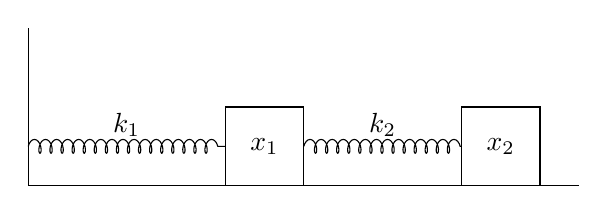
\begin{tikzpicture}
\draw (0,2) -- (0,0) -- (7,0); 

\draw[decorate,decoration={coil,segment length=4pt}] (0,0.5)   -- (2.5,0.5)
node [midway,above] {$k_1$};
\draw (2.5,0) rectangle (3.5,1); \draw (3,0.5) node {$x_1$};
\draw[decorate,decoration={coil,segment length=4pt}] (3.5,0.5)   -- (5.5,0.5)
node [midway,above] {$k_2$};
\draw (5.5,0) rectangle (6.5,1);
\draw (6,0.5) node {$x_2$};
\end{tikzpicture}
\end{center}
where $x_1$ and $x_2$ are the positions of the masses $m_1$ and $m_2$ relative to the unstretched spring positions and $k_1$ and $k_2$ are the spring constants of the two springs. 

The mass spring system above can be modeled using the 2nd order system of differential equations.  
\begin{align*}
m_1 x_1 '' & = - k_1 x_1 + k_2 (x_2-x_1) \\
m_2 x_2 '' & = - k_2 (x_2-x_1) .
\end{align*}

This can be written in matrix form as 
%
\begin{align*}
M \vec{x}'' & = K\vec{x} 
\end{align*}
with 
\begin{align*}
M & = \begin{bmatrix}
m_1 & 0 \\ 0 & m_2 
\end{bmatrix}
&
K & =\begin{bmatrix}
-(k_1+k_2) & k_2 \\ -k_2 & k_1 
\end{bmatrix}
\end{align*}
where $M$ is the mass matrix and $K$ is called the stiffness matrix, which can take other forms depending on the connectedness of the spring system. 

Since $M$ is nonsingular, we can find $M^{-1}$ and write the system above as:
%
\begin{align*}
\vec{x}'' & = A \vec{x}
\end{align*}
%
where $A = M^{-1} K$. 


\subsection{Solutions of $\vec{x}'' = A\vec{x}$}

Let $v$ be an eigenvector of $A$, with eigenvalue $\lambda = \alpha^2$, then $\vec{x} =\vec{v}(c_1e^{\alpha t} + c_2 e^{-\alpha t})$ is a solution.  

\begin{align*}
\vec{x}'' & = \alpha^2 \vec{v} (c_1 e^{\alpha t}+ c_2 e^{-\alpha t}) \\
& = A \vec{v}(c_1e^{\alpha t} + c_2 e^{-\alpha t})
\end{align*}

if $\lambda <0$, then the $\lambda = - \omega^2$ and the solution is:
%
\begin{align*}
\vec{x} & = \vec{v} (a \cos \omega t + b \sin \omega t) 
\end{align*}

If $\lambda = 0$ is an eigenvalue of $A$ with corresponding eigenvector $\vec{v}_0$, then the part of the solution associate with this is:
%
\begin{align*}
\vec{x}(t) & = (a_0 + b_0 t) \vec{v}_0
\end{align*}

\begin{theorem}
If the $n \times n$ matrix $A$ has distinct negative eigenvalues \\$-\omega_1^2, -\omega_2^2, \ldots, -\omega_n^2$ with associated real eigenvectors, then a general solution to 
%
\begin{align*}
\vec{x''} & = A x 
\end{align*}
is given by
\begin{align*}
\vec{x} & = \sum_{i=1}^n (a_i \cos \omega_i t + b_i \sin \omega_i t)\vec{v}_i
\end{align*}
where $a_i$ and $b_i$ arbitrary constants.  

If $\lambda = 0$ is an eigenvalue of $A$ with corresponding eigenvector $\vec{v}_0$, then the part of the solution associate with this is:
%
\begin{align*}
\vec{x}(t) & = (a_0 + b_0 t) \vec{v}_0
\end{align*}

\end{theorem}

\begin{example}
Consider the mass-spring system above with $m_1=1$, $m_2=2$,  $k_1 = 1$, and $k_2 = 2$, then the mass matrix and stiffness matrix are:
%
\begin{align*}
M & = 
\begin{bmatrix}
1 & 0 \\ 0 &  2
\end{bmatrix} & 
K & = \begin{bmatrix}
-3 & 2 \\ -2 & 4 \end{bmatrix}
\end{align*}
resulting in the system:

\begin{align*}
\vec{x}'' & = \begin{bmatrix}
-3 & 2 \\ -1 & 2 
\end{bmatrix} \vec{x} 
\end{align*} 

The eigenvalues and eigenvectors are:
%
\begin{align*}
\lambda_1 & = -4 & \vec{v}_1 & = (-2,1)^T \\
\lambda_2 & = -1 & \vec{v}_2 & = (1,1)^T
\end{align*}

Therefore the solution is:
%
\begin{align}
\vec{x} & = (a_1 \cos 2t + b_1 \sin 2t) \begin{bmatrix}
-2 \\ 1 
\end{bmatrix} + (a_2 \cos t + b_2 \sin t) \begin{bmatrix}
1 \\1
\end{bmatrix} \label{eq:mass:spring:soln}
\end{align}

Next, let's find the values of the $a$'s and $b$'s if $x_1=1$ and $x_2=2$ when $t=0$ or
%
\begin{align*}
\vec{x}(0) = \begin{bmatrix}
1 \\ 2
\end{bmatrix}
\end{align*}
and $\vec{x}'(0)=\vec{0}$.  First use the initial value $\vec{x}(0)$ in (\ref{eq:mass:spring:soln}), 
%
\begin{align*}
\begin{bmatrix}
1 \\ 2 
\end{bmatrix} & = a_1 \begin{bmatrix}
-2 \\ 1
\end{bmatrix} + a_2 \begin{bmatrix}
1 \\ 1
\end{bmatrix}
\end{align*}
and this is true when $a_1=1/3$ and $a_2=5/3$.  To find $b_1$ and $b_2$, differentiate (\ref{eq:mass:spring:soln}), 
%
\begin{align*}
\vec{x}'(t) & = (-2a_1 \sin 2t + 2b_1 \cos 2t ) \begin{bmatrix}
-2 \\ 1
\end{bmatrix} + (-a_2 \sin t + b_2 \cos t) \begin{bmatrix}
1 \\ 1 
\end{bmatrix} \intertext{and evaluate it at $t=0$}
\vec{x}'(0) = \begin{bmatrix}
0 \\ 0
\end{bmatrix} & = 2b_1 \begin{bmatrix}
-2 \\ 1 
\end{bmatrix} + 2b_2 \begin{bmatrix}
 1 \\ 1
\end{bmatrix}
\end{align*}
or $b_1=0$ and $b_2=0$.  The solution with the given initial condition, 
%
\begin{align*}
\vec{x}(t)  &= \frac{1}{3} \cos 2t \begin{bmatrix}
-2 \\ 1 
\end{bmatrix} + \frac{5}{3} \cos t  \begin{bmatrix}
1 \\ 1 
\end{bmatrix}
\end{align*}
The value of $x_1$ and $x_2$, the position of the two masses are the first and second components.  A plot of these two are:
%
\begin{center}
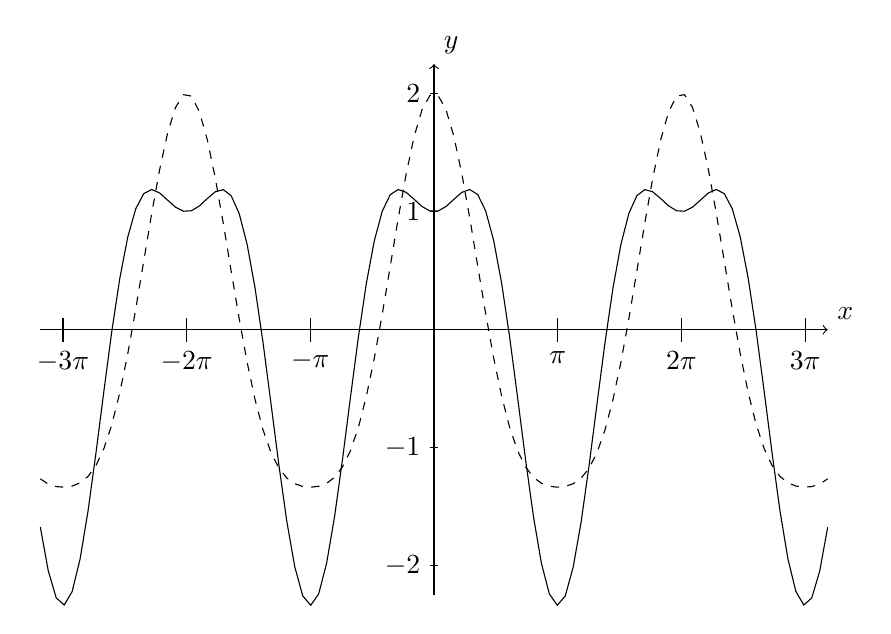
\begin{tikzpicture}[xscale=0.5,yscale=1.5]
\draw[->] (-10,0) -- (10,0) node [above right] {$x$};
\draw[->] (0,-2.25) -- (0,2.25) node [above right] {$y$}; 

% this draws all the fractional multiples of pi

%\foreach \x/\num/\den/\neg in {0.5*pi/\pi/2/,1.5*pi/3\pi/2/,-0.5*pi/\pi/2/-,-1.5*pi/3\pi/2/-} \draw ({\x},0.1) -- ({\x},-0.1) node [below] {$\neg \frac{\num}{\den}$}; 

% this draws all non fractional multiples of pi

\foreach \x/\val in {pi/\pi,2*pi/2\pi,3*pi/3\pi,-pi/-\pi,-2*pi/-2\pi,-3*pi/-3\pi} 
\draw ({\x},0.1) -- ({\x},-0.1) node [below] {$\val$}; 

\foreach \y in {-2,-1,1,2} \draw (0.1,\y) -- (-0.1,\y) node [left] {$\y$};


\draw plot[domain=-10:10,samples=100] (\x,{-2/3*cos(2*\x r)+5/3*cos(\x r)}); 
\draw[dashed] plot[domain=-10:10,samples=100] (\x,{1/3*cos(2*\x r)+5/3*cos(\x r)}); 

\end{tikzpicture}
\end{center}




\end{example}

